\documentclass{amsart}

\usepackage[T1]{fontenc}
\usepackage{enumerate, amsmath, amsfonts, amssymb, amsthm, mathrsfs, wasysym, graphics, graphicx, xcolor, url, hyperref, hypcap, shuffle, xargs, multicol, overpic, pdflscape, multirow, hvfloat, minibox, accents, array, multido, xifthen, a4wide, ae, aecompl, blkarray, pifont, mathtools, etoolbox, dsfont}
\usepackage{marginnote}
\hypersetup{colorlinks=true, citecolor=darkblue, linkcolor=darkblue}
\usepackage[all]{xy}
\usepackage[bottom]{footmisc}
\usepackage{tikz}
%\usepackage{tkz-graph}
%\usepackage{tikz-qtree}
\usetikzlibrary{trees, decorations, decorations.markings, shapes, arrows, matrix, calc, fit, intersections, patterns, angles, cd}
\usepackage[external]{forest}
%\tikzexternalize
\graphicspath{{figures/}}
\makeatletter\def\input@path{{figures/}}\makeatother
\usepackage{caption}
\captionsetup{width=\textwidth}
\renewcommand{\topfraction}{1} % possibility to have one page of pictures
\renewcommand{\bottomfraction}{1} % possibility to have one page of pictures
\usepackage[noabbrev,capitalise]{cleveref}
\usepackage[export]{adjustbox}
\usepackage{ulem}\normalem

%%%%%%%%%%%%%%%%%%%%%%%%%%%%%%%%%%%%%%

% theorems
\newtheorem{theorem}{Theorem}%[section]
\newtheorem{corollary}[theorem]{Corollary}
\newtheorem{proposition}[theorem]{Proposition}
\newtheorem{lemma}[theorem]{Lemma}
\newtheorem{conjecture}[theorem]{Conjecture}
\newtheorem*{theorem*}{Theorem}%[section]
\newtheorem*{proposition*}{Proposition}%[section]
\newtheorem*{conjecture*}{Conjecture}%[section]

\theoremstyle{definition}
\newtheorem{definition}[theorem]{Definition}
\newtheorem{example}[theorem]{Example}
\newtheorem{remark}[theorem]{Remark}
\newtheorem{question}[theorem]{Question}
\newtheorem{problem}[theorem]{Problem}
\newtheorem{notation}[theorem]{Notation}
\newtheorem{assumption}[theorem]{Assumption}
\newtheorem{defprop}[theorem]{Definition/Proposition}
\newtheorem{warning}[theorem]{Warning}
\crefname{notation}{Notation}{Notations}
\crefname{problem}{Problem}{Problems}
 
% math special letters
\newcommand{\R}{\mathbb{R}} % reals
\newcommand{\N}{\mathbb{N}} % naturals
\newcommand{\Z}{\mathbb{Z}} % integers
\newcommand{\C}{\mathbb{C}} % complex
\newcommand{\I}{\mathbb{I}} % set of integers
\newcommand{\HH}{\mathbb{H}} % hyperplane
\newcommand{\K}{\mathbb{K}} % field
\newcommand{\fA}{\mathfrak{A}} % alternating group
\newcommand{\fB}{\mathfrak{S}^\textsc{b}} % signed symmetric group
\newcommand{\cA}{\mathcal{A}} % algebra
\newcommand{\cC}{\mathcal{C}} % collection
\newcommand{\cS}{\mathcal{S}} % ground set
\newcommand{\uR}{\underline{R}} % underline set
\newcommand{\uS}{\underline{S}} % underline set
\newcommand{\uT}{\underline{T}} % underline set
\newcommand{\oS}{\overline{S}} % overline set
\newcommand{\ucS}{\underline{\cS}} % underline ground set
\renewcommand{\c}[1]{\mathcal{#1}} % caligraphic letters
\renewcommand{\b}[1]{{\boldsymbol{#1}}} % bold letters
\newcommand{\bb}[1]{\mathbb{#1}} % bb letters
\newcommand{\f}[1]{\mathfrak{#1}} % frak letters
\newcommand{\h}{\widehat} % hat letters

% math commands
\newcommand{\set}[2]{\left\{ #1 \;\middle|\; #2 \right\}} % set notation
\newcommand{\bigset}[2]{\big\{ #1 \;\big|\; #2 \big\}} % big set notation
\newcommand{\Bigset}[2]{\Big\{ #1 \;\Big|\; #2 \Big\}} % Big set notation
\newcommand{\setangle}[2]{\left\langle #1 \;\middle|\; #2 \right\rangle} % set notation
\newcommand{\ssm}{\smallsetminus} % small set minus
\newcommand{\dotprod}[2]{\left\langle \, #1 \; \middle| \; #2 \, \right\rangle} % dot product
\newcommand{\symdif}{\,\triangle\,} % symmetric difference
\newcommand{\one}{\b{1}} % the all one vector
\newcommand{\eqdef}{\mbox{\,\raisebox{0.2ex}{\scriptsize\ensuremath{\mathrm:}}\ensuremath{=}\,}} % :=
\newcommand{\defeq}{\mbox{~\ensuremath{=}\raisebox{0.2ex}{\scriptsize\ensuremath{\mathrm:}} }} % =:
\newcommand{\simplex}{\b{\triangle}} % simplex
\renewcommand{\implies}{\Rightarrow} % imply sign
\newcommand{\transpose}[1]{{#1}^t} % transpose matrix

% operators
\DeclareMathOperator{\conv}{conv} % convex hull
\DeclareMathOperator{\vect}{vect} % linear span
\DeclareMathOperator{\cone}{cone} % cone hull
\DeclareMathOperator{\inv}{inv} % inversions
\DeclareMathOperator{\ninv}{ninv} % inversions
\DeclareMathOperator{\Ima}{Im} % image
\DeclareMathOperator{\Vol}{Vol} % (mixed) volume
\DeclareMathOperator{\Hom}{Hom} % hom-spaces
\DeclareMathOperator{\Ext}{Ext} % extensions

% others
\newcommand{\ie}{\textit{i.e.}~} % id est
\newcommand{\eg}{\textit{e.g.}~} % exempli gratia
\newcommand{\Eg}{\textit{E.g.}~} % exempli gratia
\newcommand{\apriori}{\textit{a priori}} % a priori
\newcommand{\viceversa}{\textit{vice versa}} % vice versa
\newcommand{\versus}{\textit{vs.}~} % versus
\newcommand{\aka}{\textit{a.k.a.}~} % also known as
\newcommand{\perse}{\textit{per se}} % per se
\newcommand{\ordinal}{\textsuperscript{th}} % th for ordinals
\newcommand{\ordinalst}{\textsuperscript{st}} % st for ordinals
\definecolor{darkblue}{rgb}{0,0,0.7} % darkblue color
\definecolor{green}{RGB}{57,181,74} % darkblue color
\definecolor{violet}{RGB}{147,39,143} % darkblue color
\newcommand{\darkblue}{\color{darkblue}} % darkblue command
\newcommand{\defn}[1]{\textsl{\darkblue #1}} % emphasis of a definition
\newcommand{\para}[1]{\smallskip\noindent\uline{#1.}} % paragraph
\renewcommand{\topfraction}{1} % possibility to have one page of pictures
\renewcommand{\bottomfraction}{1} % possibility to have one page of pictures
%\renewcommand\labelitemi{$\diamond$} % redefine itemize default symbol

% marginal comments
\usepackage{todonotes}
\newcommand{\vincent}[1]{\todo[color=blue!30]{\rm #1 \\ \hfill --- V.}}
\newcommand{\asilata}[2][]{\todo[size=\scriptsize, color=orange!30,#1]{\rm #2 \\ \hfill --- A.}}

% lattices
\newcommand{\meet}{\wedge} % meet
\newcommand{\join}{\vee} % join
\newcommand{\bigMeet}{\bigwedge} % meet
\newcommand{\bigJoin}{\bigvee} % join
\newcommandx{\projDown}[1][1={}]{\smash{\pi_\downarrow^{#1}}} % down projection map
\newcommandx{\projUp}[1][1={}]{\smash{\pi^\uparrow_{#1}}} % up projection map
\newcommand{\con}{\mathrm{con}} % congruence

% geometry
\newcommandx{\Fan}[1][1=D]{\mathcal{F}_{#1}} % fan
\newcommand{\polytope}[1]{\mathds{#1}} % font polytope

% specific wiggly
\newcommand{\wigglyComplex}{\mathrm{WC}} % wiggly complex
\newcommand{\wigglyFlipGraph}{\mathrm{WFG}} % wiggly flip graph
\newcommand{\wigglyIncreasingFlipGraph}{\mathrm{WIFG}} % wiggly increasing flip graph
\newcommand{\wigglyLattice}{\mathrm{WL}} % wiggly lattice
\newcommand{\wigglyFan}{\mathrm{WF}} % wiggly fan
\newcommand{\wigglyhedron}{\polytope{W}} % wigglyhedron
\newcommand{\Asso}{\polytope{A}\mathsf{sso}} % associahedron

% formating the table of contents
\setcounter{tocdepth}{4}
\makeatletter
\def\l@part{\@tocline{1}{8pt}{0pc}{}{}}
\def\l@section{\@tocline{1}{4pt}{0pc}{}{}}
\makeatother
\let\oldtocpart=\tocpart
\renewcommand{\tocpart}[2]{\sc\large\oldtocpart{#1}{#2}}
\let\oldtocsection=\tocsection
\renewcommand{\tocsection}[2]{\bf\oldtocsection{#1}{#2}}
\let\oldtocsubsubsection=\tocsubsubsection
\renewcommand{\tocsubsubsection}[2]{\quad\oldtocsubsubsection{#1}{#2}}

%%%%%%%%%%%%%%%%%%%%%%%%%%%%%%%%%%%%%%

\title{Wigglyhedra for planar point sets}

\thanks{AB was partially supported by the Australian Research Council DECRA grant DE240100447. 
VP was partially supported by the Spanish project PID2022-137283NB-C21 of MCIN/AEI/10.13039/501100011033 / FEDER, UE, by the Severo Ochoa and María de Maeztu Program for Centers and Units of Excellence in R\&D (CEX2020-001084-M), by the Departament de Recerca i Universitats de la Generalitat de Catalunya (2021 SGR 00697), by the French project CHARMS (ANR-19-CE40-0017), and by the French--Austrian project PAGCAP (ANR-21-CE48-0020 \& FWF I 5788).}

\author{David Alcantara}
\address{Universidad de Cantabria}
\email{david.alcantara@unican.es}
%\urladdr{\url{}}

\author{Asilata Bapat}
\address{The Australian National University}
\email{asilata.bapat@anu.edu.au}
\urladdr{\url{https://asilata.github.io}}

\author{Vincent Pilaud}
\address{Universitat de Barcelona}
\email{vincent.pilaud@ub.edu}
\urladdr{\url{https://www.ub.edu/comb/vincentpilaud/}}

\author{Francisco Santos}
\address{Universidad de Cantabria}
\email{francisco.santos@unican.es}
\urladdr{\url{https://personales.unican.es/santosf/}}

%%%%%%%%%%%%%%%%%%%%%%%%%%%%%%%%%%%%%%

\begin{document}

\begin{abstract}
We study the wiggly complex of a planar point set.
\end{abstract}

\maketitle

%%%%%%%%%%%%%%%%%%%%%%%%%%%%%%%%%%%%%%

\section{Wiggly complex and wiggly pseudotriangulations of a planar point set}
\label{sec:wigglyComplex}

\vincent{This is copy-pasted from the wigglyhedron paper. The definition is actually inexact. To be improved.}

We consider an arbitrary point set~$P$ in the plane (neither necessarily aligned, nor necessarily in general position).

\begin{definition}
\label{def:wigglyComplexPointSet}
Fix a point set~$P$ of the plane, and an arbitrary total order~$<$ on~$P$.
A \defn{wiggly arc} is a quadruple~$(p,q,R,S)$ where~$p < q \in P$ and the sets~$R$ and~$S$ form a partition of the points of~$P$ located in the open segment joining~$p$ to~$q$.
Two wiggly arcs~$(p,q,R,S)$ and~$(p',q',R',S')$ are \defn{crossing} if 
\begin{itemize}
\item either the segments~$[p,q]$ and~$[p',q']$ cross, 
\item or~$(R \cap S') \cup (\{p,q\} \cap S') \cup (R \cap \{p',q'\}) \ne \varnothing \ne (R' \cap S) \cup (\{p',q'\} \cap S) \cup (R' \cap \{p,q\})$.
\end{itemize}
A set~$X$ of wiggly arcs is \defn{pointed} if for any~$p \in P$, the wiggly arcs of~$X$ with an endpoint at~$p$ generate a pointed cone.
The \defn{wiggly complex}~$\wigglyComplex_P$ is the simplicial complex of pairwise pointed and non-crossing subsets of wiggly arcs.
Note that the boundary wiggly arcs are irrelevant, which allows us to consider a reduced wiggly complex~$\wigglyComplex_P$ induced by internal wiggly arcs.
A \defn{wiggly pseudotriangulation} of~$P$ is a facet of~$\wigglyComplex_P$.
The \defn{wiggly flip graph}~$\wigglyFlipGraph_P$ is the adjacency graph of the facets of~$\wigglyComplex_P$.
%Note that, by construction, $\wigglyFlipGraph_P$ is regular.
See \cref{fig:wigglyComplexSquarre} for an illustration.
%
\begin{figure}[!h]
\centerline{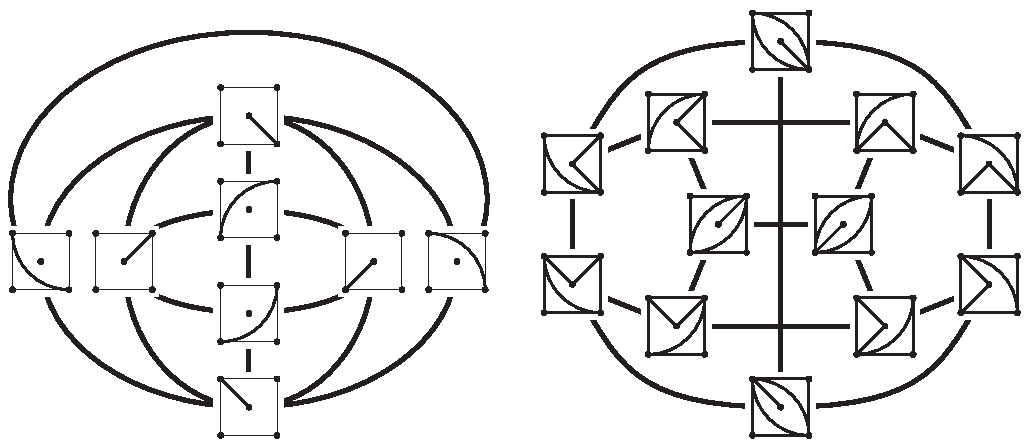
\includegraphics[scale=1]{wigglyComplexSquare}}
\caption{The wiggly complex~$\wigglyComplex_P$ (left) and the wiggly flip graph~$\wigglyFlipGraph_P$ (right) of a point set~$P$.}
\label{fig:wigglyComplexSquarre}
\end{figure}
\end{definition}

Note that \cref{def:wigglyComplexPointSet} recovers two specific situations, namely
\begin{itemize}
\item the wiggly complex of~\cite{BapatPilaud} in the case of aligned points, and
\item the pseudodissection complex of~$P$ and pseudotriangulation flip graph of~$P$ in the case of points~$P$ in general position. We refer to the original article of M.~Pocchiola and G.~Vegter~\cite{PocchiolaVegter} and to the nice survey of G.~Rote, F.~Santos and I.~Streinu~\cite{RoteSantosStreinu-pseudotriangulations}.
\end{itemize}

Observe that it is not even clear from \cref{def:wigglyComplexPointSet} that the wiggly complex~$\wigglyComplex_P$ is a pure pseudomanifold (hence that the wiggly flip graph~$\wigglyFlipGraph_P$ is well-defined).
However, we make the following ambitious conjecture.
\vincent{The goal of this new paper is to solve this conjecture.}

\begin{conjecture}
\label{conj:polytopality}
For any point set~$P$ in the plane, the wiggly complex~$\wigglyComplex_P$ is the boundary complex of a simplicial polytope.
\end{conjecture}

In \cref{conj:polytopality}, the case of aligned points is given by the wigglyhedron of~\cite{BapatPilaud}, while the case of points in general position is given by the pseudotriangulation polytope of~\cite{RoteSantosStreinu-polytope}.
This raises in particular the following question.

\begin{question}
Can the constructions of~\cite{BapatPilaud} be adapted to provide a more combinatorial construction of the polytope of pseudotriangulations~\cite{RoteSantosStreinu-polytope}, that would only depend on the order type (\aka oriented matroid~\cite{BjornerLasVergnasSturmfelsWhiteZiegler}) of the point configuration?
\end{question}

Using the duality between lines in the plane and points in the M\"obius strip, the pseudotriangulations of~\cite{PocchiolaVegter,RoteSantosStreinu-pseudotriangulations} were interpreted in~\cite{PilaudPocchiola} as pseudoline arrangements on sorting networks.
It is natural to look for the analogue of this interpretation in the wiggly setting.

\begin{question}
Is there a dual interpretation of wiggly pseudotriangulations as some sort of pseudoline arrangements? 
\end{question}

This dual interpretation enables \cite{PilaudPocchiola} to consider the pseudotriangulations of~\cite{PocchiolaVegter,RoteSantosStreinu-pseudotriangulations} and the multitriangulations of~\cite{PilaudSantos-multitriangulations} under the same roof, and to define multi-pseudo-triangulations.
The extension to the wiggly case is a natural question.

\begin{question}
Is there a multi wiggly complex?
\end{question}

Moreover, pseudoline arrangements on sorting networks can also be interpreted as (type~$A$) subword complexes of~\cite{KnutsonMiller-subwordComplex}, which in turn extend to arbitrary finite Coxeter group.
See \cite{Stump, CeballosLabbeStump} for the study of subword complexes corresponding to cluster complexes and multi-cluster complexes.

\begin{question}
Can the wiggly complex be extended to arbitrary finite Coxeter groups?
\end{question}

%\begin{question}
%\begin{itemize}
%\item Is there a dual interpretation of wiggly pseudotriangulations as some sort of pseudoline arrangements? 
%\item Is there a multi wiggly complex?
%\item Can this interpretation be extended to other finite Coxeter groups?
%\end{itemize}
%\end{question}

Finally, it is natural to consider the extension of~\cite[Conj.~44]{BapatPilaud}.

\begin{question}
\label{qu:Hamiltonian}
Is the wiggly flip graph~$\wigglyFlipGraph_P$ Hamiltonian for any point set~$P$ in the plane?
\end{question}

%%%%%%%%%%%%%%%%%%%%%%%%%%%%%%%%%%%%%%

%\clearpage
\addtocontents{toc}{ \vspace{.1cm} }
\bibliographystyle{alpha}
\bibliography{wigglyhedra}
\label{sec:biblio}

\end{document}

% Local Variables:
% TeX-command-extra-options: "-pvc"
% End:
